\documentclass{article}

\usepackage[utf8x]{inputenc}
\usepackage[english,russian]{babel}
\usepackage{cmap}
\usepackage{commath}
\usepackage{amsmath}
\usepackage{amsfonts}
\usepackage{mathtools}
\usepackage{amssymb}
\usepackage{parskip}
\usepackage{titling}
\usepackage{color}
\usepackage{hyperref}
\usepackage{cancel}
\usepackage{enumerate}
\usepackage{multicol}
\usepackage{graphicx}
\usepackage[font=small,labelfont=bf]{caption}
\usepackage[a4paper, left=2.5cm, right=1.5cm, top=2.5cm, bottom=2.5cm]{geometry}

\graphicspath{ {./images/} }
\setlength{\droptitle}{-3cm}
\hypersetup{ colorlinks=true, linktoc=all, linkcolor=blue }
\pagenumbering{arabic}

\begin{document}
    \subsection{Функция, обратная степенной}

    \(y = \sqrt[n]{x} = x^{\frac{1}{n}}, n \in \mathbb{N} \)

    Эта функция обратна к \( y = x^n, x \geq 0 \)

    \( y = \sqrt[3]{x} = x^{\frac{1}{3}} \neq x^{\frac{2}{6}} = (\sqrt[6]{x})^2 \)

    \begin{enumerate}
        \item О.О. \( x \geq 0 \)
        \item О.З. \( y \geq 0 \)
        \item Непрерывная на О.О. (как обратная к непрерывной)
        \item Монотонно возрастающая (как обратная к возрастающей)
        \item При \(n_1 > n_2\)
        \begin{enumerate}
            \item \(x^{\frac{1}{n_1}} > x^{\frac{1}{n_2}}\ 0 \leq x < 1\)
            \item \( x^{\frac{1}{n_1}} < x^{\frac{1}{n_2}}\ x > 1 \)
        \end{enumerate}
    \end{enumerate}

   \subsection{Функция вида \(x^{-n}\)}

    \( y = \frac{1}{x^n} = x^{-n}, n \in \mathbb{N}\)

    \begin{enumerate}
        \item О.О. \( x \in \mathbb{R} \backslash \{0\} \)
        \item Непрерывна на О.О.(как произведение непрерывной на \(\mathbb{R} \backslash \{0\} \)
        \item \( x > 0 \) монотонно убывающая
        
        \( x_2 > x_1 \)

        \( \frac{1}{x_2^n} - \frac{1}{x_1^n} = \frac{x_1^n - x_2^n}{x_2^n x_1^n} < 0 \)
        \item При \( n = 2k:\ y = \frac{1}{x^{2k}} \) --- четная
        
        При \( n = 2k + 1:\ y = \frac{1}{x^{2k + 1}} \) --- нечетная
        
        \item \(\lim_{x \rightarrow 0+} \frac{1}{x^n} = +\infty\)

            \(\lim_{x \rightarrow +\infty} \frac{1}{x^n} = 0\)

            \(x = 0\) --- вертикальная асимптота\\
            \(y = 0\) --- горизонтальная асимптота
        \item \(m > n\) \(\frac{1}{x^m}\) и \(\frac{1}{x^n}\)
            \begin{enumerate}
                \item \(x > 1\) \(x^m > x^n > 1 \Rightarrow \frac{1}{x^m} < \frac{1}{x^n}\)
                \item \(0 < x < 1\) \(0 < x^m < x^n \Rightarrow \frac{1}{x^m} > \frac{1}{x^n}\)
            \end{enumerate}
    \end{enumerate}

    \subsection{Степенная функция с рациональным показателем}

    \textbf{Определение.} \( y = x^r,\ r \in \mathbb{Q} \)

    \( y = x^r = x^{\frac{p}{q}} = (\sqrt[q]{x})^p = (x^p)^{\frac{1}{q}} \)

    \begin{enumerate}
        \item О.О.
        \begin{enumerate}
            \item \( r > 0,\ x \geq 0\)
            \item \( r < 0,\ x > 0\)
            \item \( r = 0,\ x \neq 0\ (y = 1)\)
        \end{enumerate}
        \item О.З.
        \begin{enumerate}
            \item \( r > 0 \)
                        
            \( y \geq 0 \)
            \item \( r < 0 \)
            
            \( y > 0 \)
            \item \(r = 0\)

            \(y = 1\)
        \end{enumerate}
        \item Непрерывная (как композиция непрерывных \( x^{\frac{p}{q}} = (\sqrt[q]{x})^p \))
        \item 
        \begin{enumerate}
            \item \(r > 0\)
            
            \(\lim_{x \rightarrow +\infty} x^r = +\infty\)
        
            \(\lim_{x \rightarrow 0} x^r = 0\)

            \item \(r < 0\)
            
            \(\lim_{x \rightarrow +\infty} x^r = 0\)

            \(\lim_{x \rightarrow 0+} x^n = +\infty\)
        \end{enumerate}
        \item Монотонность
        \begin{enumerate}
            \item \( r > 0 \) возрастает (как композиция возрастающих)
            \item \( r < 0 \) убывает (как композиция убывающей и возрастающей) 
        \end{enumerate}
    \end{enumerate}
    
    \section{Показательные функции}

    \subsection{Показательная функция рационального аргумента}

    \( y = x^r,\ x > 0 \textrm{ или } x \geq 0\)

    Фиксируем \( x = a (a > 0)\) и начинаем менять \(r \in \mathbb{Q}\). \(r\) --- показатель \(a \Rightarrow y = a^r\) --- показательная функция.

    \(y = a^r,\ r \in \mathbb{Q}\ y: \mathbb{Q} \rightarrow \mathbb{R}\ r = \frac{p}{q}\)

    \textbf{Свойства.}
    
    \begin{enumerate}
        \item О.З. \(y = a^r\ y > 0\)
        
        \(\uparrow\) Т.к. \(y=a^r\), т.к. \(\forall a > 0,\ a^p > 0,\ \forall b > 0\ \sqrt[q]{b} > 0;\ y = \sqrt[q]{a^p} > 0\ \downarrow\)
        
        \item Верны равенства:
        \begin{enumerate}
            \item \( (ab)^n = a^nb^n \)
            \item \( (\frac{a}{b})^n = \frac{a^n}{b^n} \)
            \item \( a^rs^s = a^{r+s} \)
            \item \( \frac{a^r}{a^s} = a^{r-s} \)
            \item \( (a^r)^s = a^{rs} \)
        \end{enumerate}
        \item Монотонность:
        \begin{enumerate}
            \item \(a > 1\)

            Функция монотонно возрастает.
            
            \(r_2 > r_1\)

            \(a^{r_2} - a^{r_1} = a^{r_1}_{1) > 0}(a^{r_2-r_1} - 1) > 0\)
            
            \item \( 0 < a < 1 \)
            
            Функция монотонно убывает.

            \( \frac{1}{a} > 1\)

            \( y = a^r = \frac{1}{(\frac{1}{a})^r} \Rightarrow \searrow\) (т.к. \((\frac{1}{a})^r \nearrow \))

            \item \(a = 1\ y = 1\)
            
            Функция постоянна.
        \end{enumerate}
    \end{enumerate}
    
    \subsection{Степень с иррациональным показателем}

    \( a^x,\ a > 0,\ x \) --- иррациональное

    Рассмотрим два множества:

    \( A = \{ a^r,\ r \in \mathbb{Q},\ r < x \} \);

    \( B = \{ a^r,\ r \in \mathbb{Q},\ r > x \} \).

    \begin{enumerate}
        \item \(a > 0\)
    
            Если \( r_1 < x < r_2 \), то в случае \( a > 1\ \forall r_1, r_2:\ a^{r_1} < a^{r_2} \), т.е. \(B\) правее \(A\).

            Далее \( a > 1 \)
            
            \(\Rightarrow\ \exists\) хотя бы одно разделяющее число для \(A\) и \(B\) \(\exists c :\ a^{r_1} < c < a^{r_2}\)

            Покажем, что \(c\ \exists !\)

            Если \(\exists\) система сколь угодно малых разноцветных отрезков. 
            
            \([a^{r_1}; a^{r_2}]:\ d \rightarrow 0\) ($d$ --- длина отрезка)
            
            Для \(x\ :\ \exists\)

            \(\frac{l}{10^n};\ \frac{l+1}{10^n}:\ \)

            \(\frac{l}{10^n} < x < \frac{l+1}{10^n}\)

            Докажем, что \(d = a^{r_2} - a^{r_1} \rightarrow 0\) 

            \( r_2 - r_1 = \frac{l + 1}{10^n} - \frac{l}{10^n} = \frac{1}{10^n} < \frac{1}{n} \)

            \( 10^n = (1 + 9)^n > 1 + 9n > n \)

            \( a^{r_2} - a^{r_1} = a^{r_1}(a^{r_2 - r_1} - 1) = a^{r_1}(a^{\frac{1}{10^n}} - 1) < \begin{cases}
                a > 1\\
                a^{\frac{1}{10^n}} < a^\frac{1}{n}
            \end{cases} < a^{r_1}(a^\frac{1}{n} - 1)\)

            \begin{enumerate}
                \item \( a^{r_1} \) ограничено сверху, например, \( a^r;\ r > x;\ a^{r_1} > 0 \)
                \item \( \lim_{n \to \infty}(a^\frac{1}{n} - 1) = 0 \) бесконечно малая последовательность
                \item \( \lim_{n \to \infty}(a^{r_1}(a^\frac{1}{n} - 1)) = 0\)
                \item \(\forall \varepsilon > 0\ \exists\ N:\ \forall n > N\ \abs{a^{r_2^n} - a^{r_1^n}} < \varepsilon\)
            \end{enumerate}
            
            Т.е \(\exists\) единственное разделяющее число \(c = a^x\) для \(A\) и \(B\).

        \item \( a = 1\) 
        
            \( y = 1 \)     

        \item \( 0 < a < 1;\ \)
        
            \(A\) и \(B\) меняются местами.
    \end{enumerate}

    \subsection{Показательная функция}
    
    \( y = a^x;\ a > 0;\ x \in \mathbb{R} \)

    \begin{enumerate}
        \item О.О. \( x \in \mathbb{R} \)

        \item О.З. \( y = a^x > 0 \), т.к.
        
        \( a > 1\ \forall x\ \exists r:\ x > r \Rightarrow a^x > a^r > 0 \)

        Аналогично для \( 0 < a < 1 \)

        \item Монотонность
        
        \begin{enumerate}
            \item \( a > 1:\ \nearrow \) 
            
            \( \uparrow \) \(x_1 < x_2\ a^{x_1} <^? a^{x_2} \)

            \( x_1, x_2 \) --- рациональные: \( a^{x_1} < a^{x_2} \) (из свойств \(a^r\))

            \( x_1 \) --- рациональное, \(x_2\) --- иррациональное: \(a^{x_1} < a^{x_2}\)  (из определения \(a^{x_2}\))
            
            \(x_2\) --- иррациональное, \(x_1\) --- рациональное: \(a^{x_1} < a^{x_2}\) (из определения \(a^x\))

            \( x_1, x_2 \) --- иррациональные: \( \exists\ x \) --- рациональное: \( x_1 < x < x_2 \Rightarrow a^{x_1} < a^x < a^{x_2} \) (из определения \(a^x\))
            \item \( a = 1:\ const \)
            \item \( 0 < a < 1:\ \searrow \)
        \end{enumerate}
        
        \item 
        \begin{enumerate}
            \item \(a > 1\)

            \(\lim_{x \to +\infty} a^x = +\infty\)
            
            \(\uparrow\) Надо \(\forall E > 0\ \exists\ \Delta:\ \forall x > \Delta\ a^x > E\)

            Значит, что 

            \( \lim_{n \to +\infty} a^n = +\infty \), т.е. \( \forall E > 0\ \exists\ N_*:\ \forall n > N_*\ a^n > E \)
            
            \(a^x \nearrow a > 1\ \forall x > n\ :\ a^x > a^n\)
            
            \(\Delta = N_* + 1\), тогда \(\forall x > N_* + 1 = \Delta\)

            \(a^x > a^{N_*+1} > E\ \downarrow\)
                        
            \item \(0 < a < 1\)

            Из п.1 \( \lim_{x \to +\infty}(a^x) = 0 = \lim_{x \to +\infty}(\frac{1}{(\frac{1}{a})^x}) \)
        \end{enumerate}

        \item
        \begin{enumerate}
            \item \( a > 1 \)
            
            \( \lim_{x \to -\infty} a^x = \lim_{y \to +\infty} a^{-y} = \lim_{y \to +\infty} \frac{1}{a^y} = 0 \)
            
            \item \( 0 < a < 1 \) 
            
            \( \lim_{x \to -\infty} a^x = +\infty \)
        \end{enumerate}
        
        \item Функция \(y = a^x\) непрерывна на \(\mathbb{R}\)

        \(\uparrow\) Надо \(\forall \varepsilon > 0\ \exists\ \delta\ :\ \forall x\ \abs{x - x_0} < \delta \Rightarrow \abs{f(x) - f(x_0)} = \abs{a^x-a^x_0} < \varepsilon\)

        \(\uparrow\) для \(x_0\ \exists\ r_1 = \frac{l}{10^n};\ r_2 = \frac{l + 1}{10^n};\ \frac{l}{10^n} \leq x_0 \leq \frac{l + 1}{10^n} \)
        
        \begin{enumerate}
            \item \( a > 1 \) Доказывали, что \( \abs{a^x - a^{x_0}} < \abs{a^{r_2} - a^{r_1}} < \varepsilon \)
        
            \(\forall x \in U_{\delta}(x_0)\ :\ U_{\delta}(x_0) \in [r_1, r_2]\)

            \item \( 0 < a < 1 \) Аналогично. \(\downarrow\)
        \end{enumerate}
        
        \item Функция \(y = a^x,\ a \neq 1\) принимает все положительные значения, т.е. \(\forall b \in (0; +\infty)\ \exists\ c:\ a^c = b\).

        Док-во следует из \(\lim_{x \to \pm \infty} a^x\) и следствия т. Больцано.

        \item График
        \begin{enumerate}
            \item \( a > 1 \)
            
            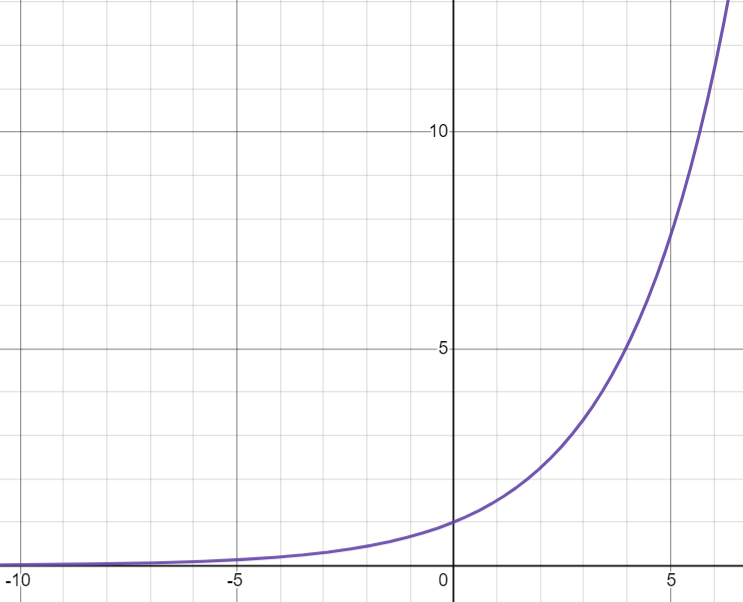
\includegraphics[scale=0.4]{11_1_6_3.png}
            \item \( 0 < a < 1 \)
            
            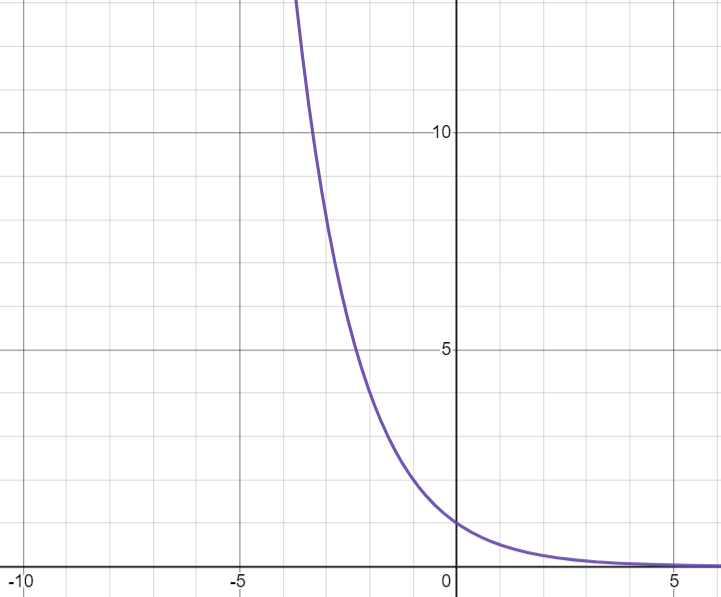
\includegraphics[scale=0.4]{11_1_6_4.png}
            \item \( a = 1 \)
            
            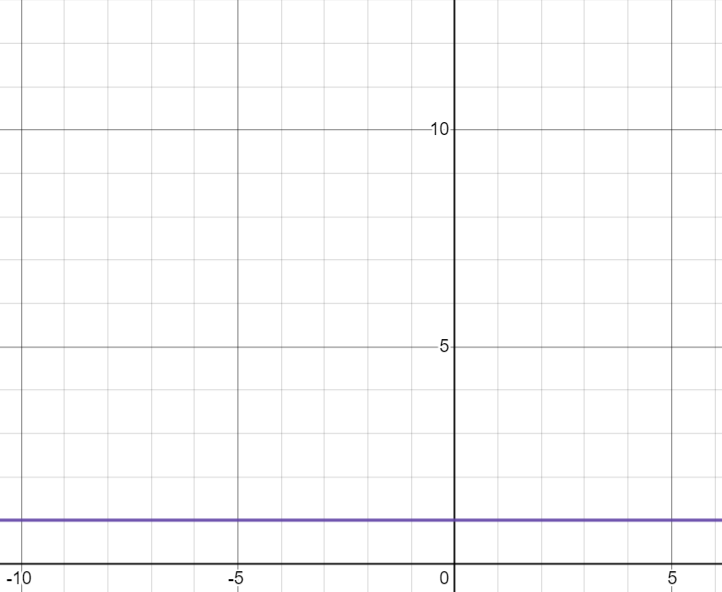
\includegraphics[scale=0.4]{11_1_6_5.png}
        \end{enumerate}

        \( \Rightarrow \) при \(a > 0;\ a \neq 1\) функция \(y = a^x\) имеет обратную(обратима).

        \item Сохраняются свойства степени:
        \begin{enumerate}
            \item \( (ab)^x = a^x b^x \)
            
            \(\uparrow\) \( \forall \) иррациональных \(x\ \exists\ r_n: r_n \xrightarrow[n \to \infty]{} x \)

            \( y = a^x \) --- непрерывная \(\Rightarrow a^x = \lim_{n \to \infty} a^{r_n}\)

            \( (ab)^x = \lim_{n \to \infty}(ab)^{r_n} = \lim_{n \to \infty}a^{r_n} b^{r_n} = \lim*\lim = a^x b^x\ \downarrow \)

            \item \((\frac{a}{b})^x = \frac{a^x}{b^x}\)
            \item \( a^x a^y = a^{x + y} \)
            \item \( \frac{a^x}{a^y} = a^{x - y} \)
            \item \( (a^x)^y = a^{xy} \)
        \end{enumerate}    
    \end{enumerate}

\end{document}